        \documentclass{article}
        \usepackage[margin=1in]{geometry}
        \usepackage{hyperref}
        \usepackage{amsmath,amsfonts,amssymb,amsthm,commath,dsfont}
        \usepackage{enumitem}
        \usepackage{framed}
        \usepackage{xspace}
        \usepackage{microtype}
        \usepackage[round]{natbib}
        \usepackage{cleveref}
        \usepackage[dvipsnames]{xcolor}
        \usepackage{graphicx}

        % following loops stolen from djhsu
        \def\ddefloop#1{\ifx\ddefloop#1\else\ddef{#1}\expandafter\ddefloop\fi}
        \def\ddef#1{\expandafter\def\csname bb#1\endcsname{\ensuremath{\mathbb{#1}}}}
        \ddefloop ABCDEFGHIJKLMNOPQRSTUVWXYZ\ddefloop
        \def\ddef#1{\expandafter\def\csname c#1\endcsname{\ensuremath{\mathcal{#1}}}}
        \ddefloop ABCDEFGHIJKLMNOPQRSTUVWXYZ\ddefloop


        \DeclareMathOperator*{\argmin}{arg\,min}
        \DeclareMathOperator*{\argmax}{arg\,max}

        \def\SPAN{\textup{span}}
        \def\tu{\textup{u}}
        \def\R{\mathbb{R}}
        \def\E{\mathbb{E}}
        \def\Z{\mathbb{Z}}
        \def\be{\mathbf{e}}
        \def\nf{\nabla f}
        \def\veps{\varepsilon}
        \def\cl{\textup{cl}}
        \def\inte{\textup{int}}
        \def\dom{\textup{dom}}
        \def\Rad{\textup{Rad}}
        \def\lsq{\ell_{\textup{sq}}}
        \def\hcR{\widehat{\cR}}
        \def\hcRl{\hcR_\ell}
        \def\cRl{\cR_\ell}
        \def\hcE{\widehat{\cE}}
        \def\cEl{\cE_\ell}
        \def\hcEl{\hcE_\ell}
        \def\eps{\epsilon}
        \def\1{\mathds{1}}
        \newcommand{\red}[1]{{\color{red} #1}}
        \newcommand{\blue}[1]{{\color{blue} #1}}
        \def\srelu{\sigma_{\textup{r}}}
        \def\vsrelu{\vec{\sigma_{\textup{r}}}}
        \def\vol{\textup{vol}}

        \newcommand{\ip}[2]{\left\langle #1, #2 \right \rangle}
        \newcommand{\mjt}[1]{{\color{blue}\emph\textbf{[M:}~#1~\textbf{]}}}
        \newcommand{\sahand}[1]{{\color{green}\emph\textbf{[Sah:}~#1~\textbf{]}}}

        \newtheorem{fact}{Fact}
        \newtheorem{lemma}{Lemma}
        \newtheorem{claim}{Claim}
        \newtheorem{proposition}{Proposition}
        \newtheorem{theorem}{Theorem}
        \newtheorem{corollary}{Corollary}
        \newtheorem{condition}{Condition}
        \theoremstyle{definition}
        \newtheorem{definition}{Definition}
        \theoremstyle{remark}
        \newtheorem{remark}{Remark}
        \newtheorem{example}{Example}

        \newenvironment{Q}
        {%
          \clearpage
          \item
        }
        {%
          \phantom{s} %lol doesn't work
          \bigskip
          \textbf{Solution.}
        }

        \title{CS 446 MJT --- Homework 1}
        \author{\emph{your NetID here}}
        \date{Version 1}

        \begin{document}
        \maketitle

        \textbf{Instructions.}
        \begin{itemize}
          \item
            Homework is due \textbf{Tuesday, February 5, at 11:59pm}; no late homework accepted.

          \item
            Everyone must submit individually at gradescope under \texttt{hw1} and \texttt{hw1code}.

          \item
            The ``written'' submission at \texttt{hw1} \textbf{must be typed}, and submitted in
            any format gradescope accepts (to be safe, submit a PDF).  You may use \LaTeX, markdown,
            google docs, MS word, whatever you like; but it must be typed!

          \item
            When submitting at \texttt{hw1}, gradescope will ask you to mark out boxes
            around each of your answers; please do this precisely!

          \item
            Please make sure your NetID is clear and large on the first page of the homework.

          \item
            Your solution \textbf{must} be written in your own words.
            Please see the course webpage for full academic integrity information.
            Briefly, you may have high-level discussions with at most 3 classmates,
            whose NetIDs you should place on the first page of your solutions,
            and you should cite any external reference you use; despite all this,
            your solution must be written in your own words.

          \item
            We reserve the right to reduce the auto-graded score for \texttt{hw1code}
            if we detect funny business (e.g., rather than implementing an algorithm,
            you keep re-submitting the assignment to the auto-grader, eventually completing
            a binary search for the answers).
            \item In this assignment, for all code unless otherwise specified please return your output as a NumPy array.

        \end{itemize}
        \begin{enumerate}
          \begin{Q}
            \textbf{Decision Trees.}

              Consider the training data given in Figure~\ref{fig:p1 training set}.
              \begin{figure}[h]
                \centering
                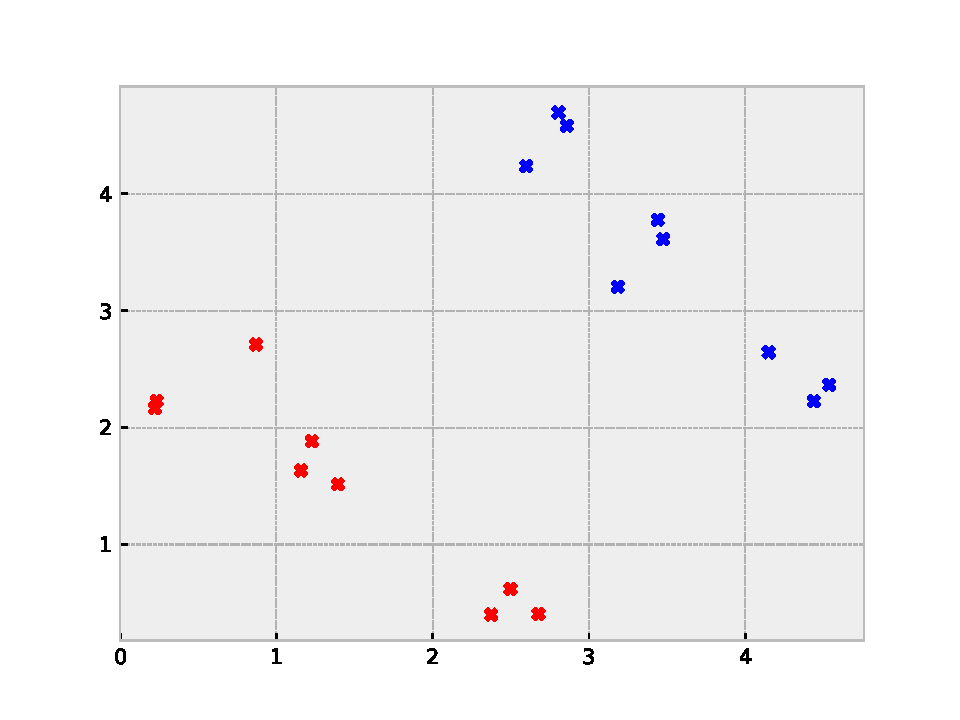
\includegraphics[width=0.6\linewidth]{figures/training.pdf}
                \caption{Training data}
                \label{fig:p1 training set}
              \end{figure}
            \begin{enumerate}
              \item Describe a decision tree of depth one with integral and axis-aligned decision boundaries for this data set, with training error at most $\frac 1 6 = .166\dots$.
              \item Describe a decision tree with integral and axis-aligned decision boundaries for this data set, with zero training error.
              \item Describe a decision tree with integral and axis-aligned decision boundaries for this data set, with zero training error such that the testing error rate is large when given the testing set of Figure~\ref{fig:p1 testing set}.
              \begin{figure}[h]
                \centering
                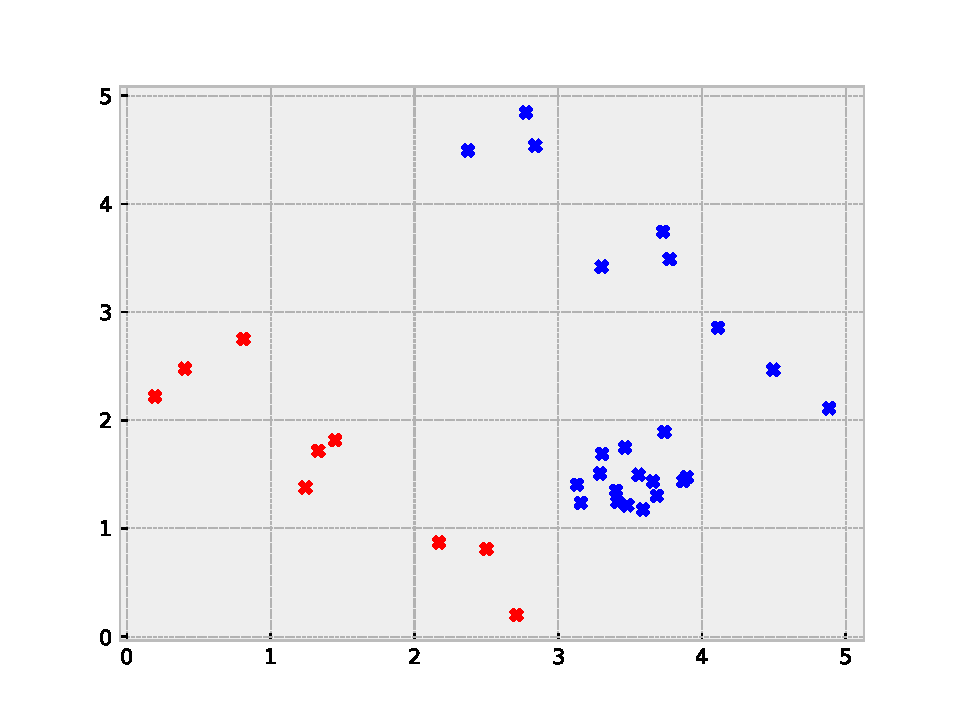
\includegraphics[width=0.6\linewidth]{figures/testing.pdf}
                \caption{Testing data}
                \label{fig:p1 testing set}
              \end{figure}
            \end{enumerate}
          \end{Q}
          \emph{(Your solution here.)}


          \begin{Q}
          \textbf{Linear Regression.}

          Recall that the empirical risk in the linear regression method is defined as $\hcR(w) := \frac{1}{2n}\sum_{i=1}^n (w^\top x_i - y_i)^2$, where $x_i \in \R^d$ is a data point and $y_i$ is an associated label.
          \begin{enumerate}
            \item Implement the linear regression method using gradient descent in \texttt{linear\_gd(X, Y, lrate, num\_iter)} function in \texttt{hw1.py}. You are given a training set \texttt{X} as input and training labels \texttt{Y} as input along with a learning rate \texttt{lrate} and maximum number of iterations \texttt{num\_iter}.  Using gradient descent find parameters $w$ that minimize the empirical risk $\hcR(w)$.  One iteration is equivalent to one full data gradient update step. Use a learning rate of \texttt{lrate} and only run for \texttt{num\_iter} iterations. Use $w = 0$ as your initial parameters, and return your parameters $w$ as output.  (Note: gradient descent will be covered in lecture 5.)
            \item Implement linear regression by setting the gradient to zero and solving for the variables, in \texttt{linear\_normal(X,Y)} function in \texttt{hw1.py}. You are given a training set \texttt{X} as input and training labels \texttt{Y} as input.  (Lectures 3-4 give a few ways to get an answer here.) Return your parameters $w$ as output.
          \item Implement the \texttt{plot\_linear()} function in \texttt{hw1.py}.  Use the provided function \texttt{utils.load\_reg\_data()} to generate a training set \texttt{X} and training labels \texttt{Y}. Plot the curve generated by \texttt{linear\_normal()} along with the points from the data set.  Return the plot as output.  Include the plot in your written submission.
          \end{enumerate}
          \end{Q}
          \emph{(Your solution here.)}


          \begin{Q}
          \textbf{Singular Value Decomposition.}

          Recall, as detailed in lecture 3,
          that for every matrix $A \in \R^{n \times d}$, there are matrices $U \in \R^{n \times n}$, $S \in \R^{n \times d}$ and $V \in \R^{d \times d}$ such that $A = U S V^\top$ and $S$ is a diagonal matrix and $U$ and $V$ are orthonormal matrices, that is $U^{-1} = U^\top$ and $V^{-1} = V^\top$ (i.e. its inverse is equal to its transpose).
          (A convenient alternative notation, as discussed in lecture, is $A = \sum_{i=1}^r s_i u_i v_i^\top$.)
          \begin{enumerate}
            \item Let $A \in \R^{n \times n}$ be a square matrix and consider its singular value decomposition $U S V^\top$ with values $s_1, \ldots, s_n$ on the diagonal of $S$. Show that $A$ is invertible if and only if $s_i \neq 0$ for all $i \in \set{1,\ldots,n}$.
            \item Show that for all $A \in \R^{n \times d}$ and all positive $\lambda \in \R_{>0}$, the matrix $(A^\top A)+\lambda I$ is invertible.
            \item Prove that $\lim_{\lambda \downarrow 0} (A^\top A + \lambda I)^{-1} A^\top \to A^+$, where $A^+$ is the pseudoinverse of the matrix $A$. That is to show that every entry of the matrix $(A^\top A + \lambda I)^{-1} A^\top$ converges to the corresponding entry in $A^+$ as $\lambda$ vanishes.
          \end{enumerate}
          \end{Q}
          \emph{(Your solution here.)}


          \begin{Q}
          \textbf{Polynomial Regression.}

          In problem 2 you constructed a linear model $w^\top x = \sum_{i=1}^d x_i w_i$.  In this problem you will use the same setup as in the previous problem, but enhance your linear model by doing a quadratic expansion of the features.  Namely, you will construct a new linear model $f_{w}$ with parameters $(w_{0}, w_{01},\dots,w_{0d},w_{11}, w_{12},\dots,w_{1d},w_{22}, w_{23},\dots,w_{2d},\dots, w_{dd})$ defined:
          	\begin{align*}
          	f_{w}(x) = w^\top \phi(x) = w_0 + \sum_{i=1}^d w_{0i} x_i + \sum_{i\leq j}^dw_{ij} x_ix_j
          	\end{align*}
          \begin{enumerate}
          \item Given a $3$-dimensional feature vector $x = (x_1,x_2,x_3)$ completely write out the quadratic expanded feature vector $\phi(x)$.
          \item Implement the \texttt{poly\_gd()} function in \texttt{hw1.py}.  The input is in the same format as it was in problem 2.  Use this training set to implement gradient descent to determine the parameters $w$.  Use $w = 0$ as your initial parameters.  Return your $w$ parameters as output.  Please return your parameters in the exact order mentioned here (bias, linear, and then quadratic).  For example, if $d = 3$ then you would return $(w_0, w_{01},w_{02},w_{03},w_{11},w_{12},w_{13},w_{22},w_{23},w_{33})
$.          \item Implement the \texttt{poly\_normal} function in \texttt{hw1.py}.  You are given the same data set as from part (b), but this time you will determine the $w$ parameters by solving the normal equations.  Return your $w$ parameters as output.  Again, return these parameters in the same order you returned them for part (b).
          \item Implement the \texttt{plot\_poly()} function in \texttt{hw1.py}.  Use the provided function \texttt{utils.load\_reg\_data()} to generate a training set \texttt{X} and training labels \texttt{Y}. Plot the curve generated by \texttt{poly\_normal()} along with the points from the data set.  Return the plot as output and include it in your written submission.  Compare and contrast this plot with the plot from problem 2.  Which model appears to approximate the data best? Provide a justification for your answer.
          \item The Minsky-Papert XOR problem is a classification problem with data set: \begin{align*}
          X = \{(-1,+1), (+1,-1), (-1,-1),(+1,+1)\}
    \end{align*}
    where the label for a given point $(x_1,x_2)$ is given by its product $x_1x_2$.  For example, the point $(-1,+1)$ would be given label $y = (-1)(1) = -1$.  Implement the \texttt{poly\_xor()} function in \texttt{hw1.py}.  In this function you will load the XOR data set by calling the \texttt{utils.load\_xor\_data()} function, and then apply the \texttt{linear\_normal()} and \texttt{poly\_normal()} functions to generate labels for the XOR points. Include a plot of contour lines that show how each model classifies points in your written submission.  You may use \texttt{contour\_plot()} in \texttt{hw1\_utils.py} to help you plot the contour lines.  As output, return both the labels for the linear model and the polynomial model in that order.  Do both models correctly classify all points?
          \end{enumerate}
          \end{Q}
          \emph{(Your solution here.)}
          \begin{Q}
    	  \textbf{Nearest Neighbor.}

          \begin{enumerate}
          \item Implement the 1-nearest neighbor algorithm in the \texttt{nn()} function in \texttt{hw1.py}. In the starter code you are given three NumPy arrays as input:
    	\begin{itemize}
    	  \item \texttt{X} - training set
    	  \item \texttt{Y} - training labels
          \item \texttt{X\_test} - testing set
          \end{itemize}
          Use the training set to determine labels for the testing set. Return the labels for the testing set as determined by your nearest neighbor implementation.
          \item Plot the Voronoi diagram of your nearest neighbor results. Use the data set returned from \texttt{utils.load\_nn\_data()} to make this plot. You may use the function \texttt{utils.voronoi\_plot()} provided to you in \texttt{hw1\_utils.py} to help generate the diagram.  There is no need to submit code for this part, only submit the plots in the written portion.
           \item Implement the \texttt{nn\_iris()} function in \texttt{hw1.py}.  Here you will use your nearest neighbor implementation on the Iris data set provided by the scikit-learn library (which can be installed via ``\texttt{pip3 install scikit-learn}'').  Use the \texttt{utils.load\_iris\_data()} function to load the data set, and then split the data set into a testing set and training set.  Take the first $30\%$ of the data set to be the testing set, and the rest of the data set to be the training set.  Run your \texttt{nn()} function on this data set and return your classification accuracy as output.  Report your classification accuracy in your written submission.
          \end{enumerate}
          \end{Q}
          \emph{(Your solution here.)}
          \begin{Q}
          \textbf{Logistic Regression.}

          Recall the empirical risk $\hcR$ for logistic regression (as presented in lectures 5-6):
          \begin{align*}
          \hcR_{\log}(w) = \frac{1}{n} \sum_{i=1}^n \ln ( 1 + \exp( - y_i w^\top x_i ) )
          \end{align*}
          Here you will minimize this risk using gradient descent.
          \begin{enumerate}
          \item In your written submission, derive the gradient descent update rule for this empirical risk by taking the gradient.  Write your answer in terms of the learning rate $\eta$, previous parameters $w$, new parameters $w'$, number of examples $n$, and training examples $x_i$.  Show all of your steps.
          \item Implement the \texttt{logistic()} function in \texttt{hw1.py}.  You are given a training set \texttt{X} as input and training labels \texttt{Y} as input along with a learning rate \texttt{lrate} and maximum number of iterations \texttt{num\_iter}.  Implement gradient descent in order to find parameters $w$ that minimize the empirical risk $\hcR_{\log}(w)$.  One iteration is equivalent to one full data gradient update step.  Return your parameters $w$ as output.  You may use PyTorch to handle the gradient computation for you.  Use $w = 0$ as your initial parameters.  Use a learning rate of \texttt{lrate} and only run for \texttt{num\_iter} iterations.
          \item Now implement the \texttt{logistic\_vs\_ols()} function in \texttt{hw1.py}.  This time you are only given the training set \texttt{X} and training labels \texttt{Y} as input.  Run \texttt{logistic(X,Y)} from part (b) taking \texttt{X} and \texttt{Y} as input to obtain parameters $w$ (use the defaults for \texttt{num\_epochs} and \texttt{lrate}).  Also run \texttt{linear\_gd(X,Y)} from problem 2 also taking \texttt{X} and \texttt{Y} as input to obtain parameters $w$.  Plot both lines generated by logistic regression and least squares along with the data \texttt{X}. Use the data set returned from the \texttt{utils.load\_logistic\_data()} function to make this plot. Which model appears to classify the data better? Provide an explanation for why you believe your choice is the better classifier for this problem.
          \end{enumerate}
          \end{Q}
          \emph{(Your solution here.)}
        \end{enumerate}


        \end{document}
